\section{Convolution}

Let $F$ and $G$ be two $n$-th order tensors where all axes of $F$ have size $d_F$ and all axes of $G$ have size $d_G$ with $d_F < d_G$.
Let $d_O = d_G - d_F + 1$.
Then the convolution $F * G$ is defined in the following way:
$$(F * G)_x := \sum\limits_{y \in [d_F]^n} F_y \cdot G_{x + d_F - y}$$
for all $x \in [d_O]^n$, where $x + d_F - y$ indicates the element-wise addition $(x + d_F - y)_i = x_i + d_F - y_i$ for $i \in [n]$.
Let
$$G'_{(x, y)} := G_{x + d_F - y}$$
for $x \in [d_O]^n, y \in [d_F]^n$.
Then
$$(F * G)_x = \sum\limits_{y \in [d_G]^n} F_y G'_{(x, y)}.$$
Let
$$P_{(x, y, z)} = \begin{cases}
        1 & \text{if } z = x + d_F - y \\
        0 & \text{else}
    \end{cases}$$
for $x \in [d_O]^n, y \in [d_F]^n, z \in [d_G]^n$.
Then
$$G'_{(x, y)} = \sum\limits_{z \in [d_G]^n} P_{(x, y, z)} G_z.$$
Therefore, convolution can be expressed as an Einsum expression:
$$(F * G) = ((\bm{s_x},\bm{s_y},\bm{s_z}),\bm{s_y}, \bm{s_z}  \rightarrow \bm{s_x}, P, F, G)$$
where $\bm{s_x},\bm{s_y},\bm{s_z} \in S^n$ use distinct symbols.

The manual computation of the design tensor $P$ is quite expensive, and therefore this expression could be inefficient.
It could lead to a more efficient computation, if this design tensor could be expressed as an \textit{outer product} of 2 or more smaller tensors.
Sadly, this is not possible.

\bigskip
\begin{proof}
    \small
    To prove this, we will first show that, if $P$ can be expressed as an outer product, then the factors also have to be scaled design tensors.
    Then we will give an example of a convolution, where $P$ can not be expressed as an outer product of design tensors.

    Let $U$ be an $m$-th order tensor, and $V$ an $(3n-m)$-th order tensor for $1 \leq m < 3n$.
    Let $\bm{s_u} \in S^{m}$ be the index string for $U$,
    and let $\bm{s_v} \in S^{3n - m}$ be the index string for $V$ such that $\bm{s_u}$ and $\bm{s_v}$ use distinct symbols.
    Then $P$ being the outer product of $U$ and $V$ means
    $$P = (\bm{s_u}, \bm{s_v} \rightarrow (\bm{s_u}, \bm{s_v}), U, V)$$
    up to reordering of axes.

    Let $u$ and $v$ be entries of $U$ and $V$ respectively, and let $\bm{i_u}$ and $\bm{i_v}$ be a multi-index of $U$ and $V$ respectively, where this value occurs.
    Then the value $u \cdot v$ occurs in $P$ at the multi-index $(\bm{i_u}, \bm{i_v})$.
    Therefore, if the sets of values contained in $U$ and $V$ are not of the form $\smallset{0, c}$ and $\smallset{0, \frac{1}{c}}$ for some $c \in \R$, then we can produce more values than $0$ and $1$ in $P$.
    Therefore $U$ and $V$ must be design tensors that were scaled by $c$ and $\frac{1}{c}$ respectively for some $c \in \R$.

    W.l.o.g. we now assume that $U$ and $V$ are both unscaled design tensors, because if
    $$P = (\bm{s_u}, \bm{s_v} \rightarrow (\bm{s_u}, \bm{s_v}), c U, \frac{1}{c} V)$$
    then
    \begin{align*}
        P & = c\cdot \frac{1}{c} \cdot (\bm{s_u}, \bm{s_v} \rightarrow (\bm{s_u}, \bm{s_v}), U, V) \\
          & = (\bm{s_u}, \bm{s_v} \rightarrow (\bm{s_u}, \bm{s_v}), U, V).
    \end{align*}

    Consider a convolution $F * G$ of vectors $F \in \R^2$ and $G \in \R^3$.
    Then
    $$(F * G)_x = \sum\limits_{y \in [2]} F_y G_{x + 2 - y}$$
    for $x \in [2]$, and
    $$P_{(x,y,z)} = \begin{cases}
            1 & \text{if } z = x + 2 - y \\
            0 & \text{else}
        \end{cases}$$
    for $x \in [2], y \in [2], z \in [3]$.
    This is illustrated in \autoref{fig:translating_inference:dft:example_p}.
    \begin{figure}
        \centering
        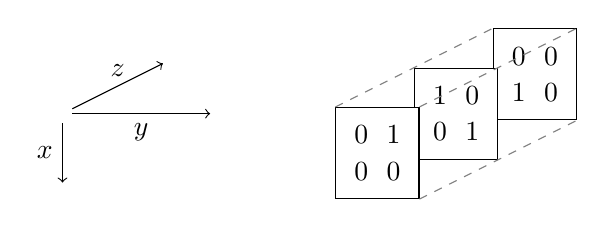
\begin{tikzpicture}
            % vertical horizontal shift
            \def\dx{1}
            \def\dy{0.5}
            % P
            \matrix[draw, fill=white] (layer_3) at (2 * \dx, 2 * \dy) {
                \node (113) {$0$}; & \node (123) {$0$}; \\
                \node (213) {$1$}; & \node (223) {$0$}; \\
            };
            \matrix[draw, fill=white] (layer_2) at (1 * \dx, 1 * \dy) {
                \node (112) {$1$}; & \node (122) {$0$}; \\
                \node (212) {$0$}; & \node (222) {$1$}; \\
            };
            \matrix[draw, fill=white] (layer_1) at (0 * \dx, 0 * \dy) {
                \node (111) {$0$}; & \node (121) {$1$}; \\
                \node (211) {$0$}; & \node (221) {$0$}; \\
            };
            \draw [dashed,gray](layer_1.north west) -- (layer_3.north west);
            \draw [dashed,gray](layer_1.north east) -- (layer_3.north east);
            \draw [dashed,gray](layer_1.south east) -- (layer_3.south east);
            % the directions
            \node (d0) at (-4 * \dx, \dy) {};
            \node (dx) at (-4 * \dx, -\dy) {};
            \node (dy) at (-4 * \dx + 2 * \dx, \dy) {};
            \node (dz) at (-4 * \dx + 1.4 * \dx, 2.4 * \dy) {};
            \draw[->] (d0) to node[midway, left] {$x$} (dx);
            \draw[->] (d0) to node[midway, below] {$y$} (dy);
            \draw[->] (d0) to node[midway, above] {$z$} (dz);
        \end{tikzpicture}
        \caption{$P$ for $F \in \R^2$ and $G \in \R^3$}
        \label{fig:translating_inference:dft:example_p}
    \end{figure}

    Now, the only two possibilities for $m$ are $m = 1$ and $m = 2$, because $n = 1$ and therefore $1 \leq m < 3$.
    This means, $U$ and $V$ are a matrix and a vector.
    W.l.o.g. we assume that $U$ is a matrix and $V$ is a vector.
    Then for $U$ to be a matrix and a factor of $P$, there are only three possibilities:
    \begin{align*}
        P_{xyz} & = U_{xy} V_z, \\
        P_{xyz} & = U_{xz} V_y, \\
        P_{xyz} & = U_{yz} V_x.
    \end{align*}
    In the first case, it has to hold that $U_{xy} = 1$ where $P_{xyz} = 1$ for any $z \in [3]$,
    because otherwise, no design tensor $V$ could produce the entry $P_{xyz} = 1$.
    For the other two cases, the analogue fact holds:
    all the entries, where missing index exists such that $P_{xyz} = 1$, have to hold one as well.
    And unless $V$ is full of zeros (which it cannot be), the converse is true as well,
    meaning if all entries of the missing index hold $P_{xyz} = 0$, then the entry in $U$ also has to hold zero.
    Therefore there is only possibility for $U$ for each of the cases, which are illustrated in \autoref{fig:translating_inference:dft:example_us}:
    \begin{align*}
        P_{xyz} & = U_{xy} V_z & U & = \begin{pmatrix} 1 & 1 \\ 1 & 1 \end{pmatrix} \\
        P_{xyz} & = U_{xz} V_y & U & = \begin{pmatrix} 1 & 1 & 0 \\ 0 & 1 & 1 \end{pmatrix} \\
        P_{xyz} & = U_{yz} V_x & U & = \begin{pmatrix} 0 & 1 & 1 \\ 1 & 1 & 0 \end{pmatrix}
    \end{align*}
    \begin{figure}
        \centering
        \begin{subfigure}{0.3\textwidth}
            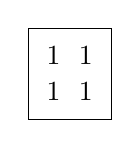
\begin{tikzpicture}
                % vertical horizontal shift
                \def\dx{1}
                \def\dy{0.5}
                % U
                \matrix[draw, fill=white] (layer_1) at (0 * \dx, 0 * \dy) {
                    \node {$1$}; & \node {$1$}; \\
                    \node {$1$}; & \node {$1$}; \\
                };
            \end{tikzpicture}
            \caption{$P_{xyz} = U_{xy} V_z$}
        \end{subfigure}
        \begin{subfigure}{0.3\textwidth}
            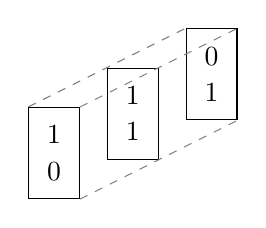
\begin{tikzpicture}
                % vertical horizontal shift
                \def\dx{1}
                \def\dy{0.5}
                % U
                \matrix[draw, fill=white] (layer_3) at (2 * \dx, 2 * \dy) {
                    \node {$0$}; \\
                    \node {$1$}; \\
                };
                \matrix[draw, fill=white] (layer_2) at (1 * \dx, 1 * \dy) {
                    \node {$1$}; \\
                    \node {$1$}; \\
                };
                \matrix[draw, fill=white] (layer_1) at (0 * \dx, 0 * \dy) {
                    \node {$1$}; \\
                    \node {$0$}; \\
                };
                \draw [dashed,gray](layer_1.north west) -- (layer_3.north west);
                \draw [dashed,gray](layer_1.north east) -- (layer_3.north east);
                \draw [dashed,gray](layer_1.south east) -- (layer_3.south east);
            \end{tikzpicture}
            \caption{$P_{xyz} = U_{xz} V_y$}
        \end{subfigure}
        \begin{subfigure}{0.3\textwidth}
            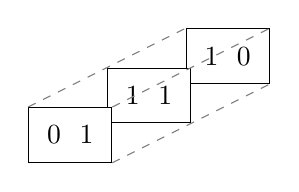
\begin{tikzpicture}
                % vertical horizontal shift
                \def\dx{1}
                \def\dy{0.5}
                % U
                \matrix[draw, fill=white] (layer_3) at (2 * \dx, 2 * \dy) {
                    \node {$1$}; & \node {$0$}; \\
                };
                \matrix[draw, fill=white] (layer_2) at (1 * \dx, 1 * \dy) {
                    \node {$1$}; & \node {$1$}; \\
                };
                \matrix[draw, fill=white] (layer_1) at (0 * \dx, 0 * \dy) {
                    \node {$0$}; & \node {$1$}; \\
                };
                \draw [dashed,gray](layer_1.north west) -- (layer_3.north west);
                \draw [dashed,gray](layer_1.north east) -- (layer_3.north east);
                \draw [dashed,gray](layer_1.south east) -- (layer_3.south east);
            \end{tikzpicture}
            \caption{$P_{xyz} = U_{yz} V_x$}
        \end{subfigure}
        \caption{Possiblities for $U$ in the factorization of $P$}
        \label{fig:translating_inference:dft:example_us}
    \end{figure}

    Therefore, the multiplication with $V$ has to spread out the ones across different values of the missing index,
    which is not possible, because depending on the entries of $V$ on the missing index:
    \begin{itemize}
        \item if $V$ is one at a value of the missing index, then $P$ is a copy of $U$ at this value of the missing index, and
        \item if $V$ is zero at a value of the missing index, then $P$ is zero at this value of the missing index.
    \end{itemize}

    Therefore, there is no factorization of $P$ when $F \in \R^2$ and $G \in \R^3$,
    which means $P$ can not generally be expressed as an outer product of two lower-order tensors.
\end{proof}